\subsection{Използвани технологии}


\begin{enumerate}
 \itemЗа разработката на приложението е използвана интегрираната среда за разработка на софтуер \textit{Visual Studio 2017}. 
 \itemИзползваният програмен език е \textit{C Sharp}. 
 \itemЗа визуализацията на примитиви в 3D е използвана библиотеката с отворен код \textit{Helix Toolkit 3D}. Позволява достъп до вече настроен viewport, както и някои базови за работата с 3D обекти функции – ротация, транслация и скалиране.
 \item \textit{WPF} 
 \itemЗа олеснена работа със структурата от данни граф е използвана библиотеката с отворен код \textit{QuickGraph}. \textit{BidirectionalGraph<V,E>} е конкретната имплементация на граф използвана в проекта.  Тя представлява неориентиран граф, Използва се, за да се репрезентират обектите като върхове, а разстоянията измерени между обектите като дъги между върховете. Два обекта са свързани с не ориентирана дъга с тегло равно на разстоянието между двата обекта, ако няма измерение на разстоянието между обектите то тогава дъга между двата върха няма.
 \itemЗа тестване на програмата в реални условия са използвани 4 бр. ултразвуков трансмитери и 1 бр. ултразвук получател, с производител : Hexamite. Устройствата са предоставени от др. Димитър Минчев
\end{enumerate}

\subsection{Обосновка за използвани технологии}

\begin{enumerate}
    \item Visual Studio предоставя мощна интегрирана среда за писане на код, компилиране, изпълнение, дебъгване (както за високо така и за машинно ниво), тестване на приложения, дизайн на потребителски интерфейс (форми, диалози, уеб страници, визуални контроли и други), моделиране на данни, моделиране на класове, изпълнение на тестове, пакетиране на приложения и стотици други функции. Могат да се добавят и плъгини, които повишават функционалността на почти всяко ниво – включително добавянето на поддръжка за source-control системи (като Subversion и Visual SourceSafe), добавяне на нови инструменти като редактори и визуални дизайнери за domain-specific languages или инструменти за други аспекти (като например: Team Foundation Server, Team Explorer). \cite{vs}
    
    \item C Sharp е широкоприет програмен език, които заимства от различни парадигми в програмирането - функционално, обектно-ориентирано и т.н. Разработен е от Microsoft, което позволява лесна интеграция с останалите инструменти, които се използват в настоящата дипломна работа. C Sharp се счита за 5-тия най-популярене зик за програмиране според класацията на TIOBE. [фиг. \ref{fig:prog}]
    
    \item XAML e декларативен маркъп език използван за иницализиране на структурирани стойности и обекти. Използва се за оформление на структурата на софтуерни приложение. Разработен е от Microsoft и е единственият подържан маркъп език, който се подържа от платформата WPF. В настоящата дипломна работа, той се използва, за да се структурира визуално информацията използвана в софтуерната програма, която бе разработена.
    
    \item WPF ( Windows Presentation Foundation ) \cite{wpf} е набор от инструменти, които олесняват разработката на Windows Desktop приложения Използва се за главно за разработка на приложения за персоналния компютър, но може да бъде използван и в уеб среда. Често е предпочитан пред останалите варианти заради стабилността на инструментите и това че разработвания софтуер е независим от интернет връзка. Той подържа работа с 3D примитиви използвайки Direct X. \cite{wpfUsage}
    
    \item Helix Toolkit надгражда вградените в WPF функционалности за работа с 3D обекти. Въпреки, че не може да се сравнява по мощност с напредналите инструменти за разработка на 3D модели, Helix Toolkit съдържа достатъчно функционалности, за да бъде достатъчна за работа с обекти в 3D. Съдържа оптимизирани имплементации на често използвани операции обработката на визуална информация ( скалиране , ротация и транслация). Съдържа помощни обекти, които позоволяват да се упражнява контрол над камерата. Съдържа помощни функции за контрол над осветлението във виртуалното пространство. \cite{helix}
    
    \item QuickGraph предлага стабилни имплементации на структурата от данни граф за платформата за разработка .NET. Това включва насочен/ненасочен граф. Имплементирани са често използвани алгоритми като търсене в дълбочина, търсене в дълбочина , A* търсене и т.н. \cite{quickgraph}

    
\end{enumerate}


\begin{figure}
    \centering
    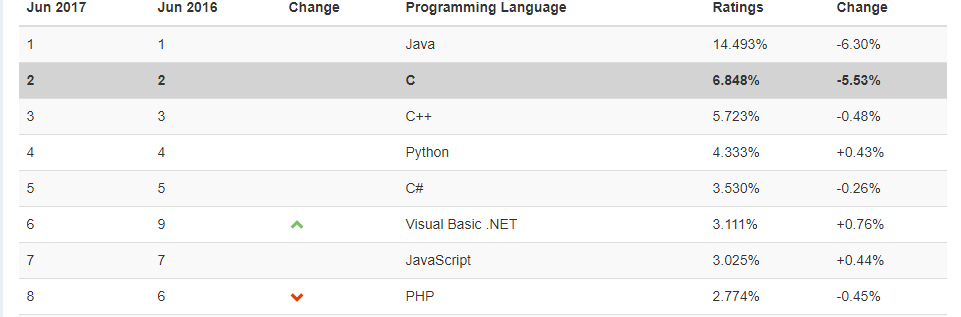
\includegraphics{programmingLanguage}
    \caption{Езици за програмиране сортирани низходящо}
    \label{fig:prog}
\end{figure}
